\section{Introduction}

    The goal of this experiment series is to build a spectrometer using household objects by making use of the wave character of light.
    % Interference double-silt source: https://wiki.anton-paar.com/ch-de/doppelspaltexperiment/
    % Interference grating source: https://www.grund-wissen.de/physik/optik/wellenoptik.html
    % Grating constant source: https://ieeexplore.ieee.org/stamp/stamp.jsp?tp=&arnumber=5547333&tag=1 (eth network)
    
    \begin{minipage}{0.99\linewidth}
        \begin{minipage}{0.5\linewidth}
            \begin{figure}[H]
                \centering
                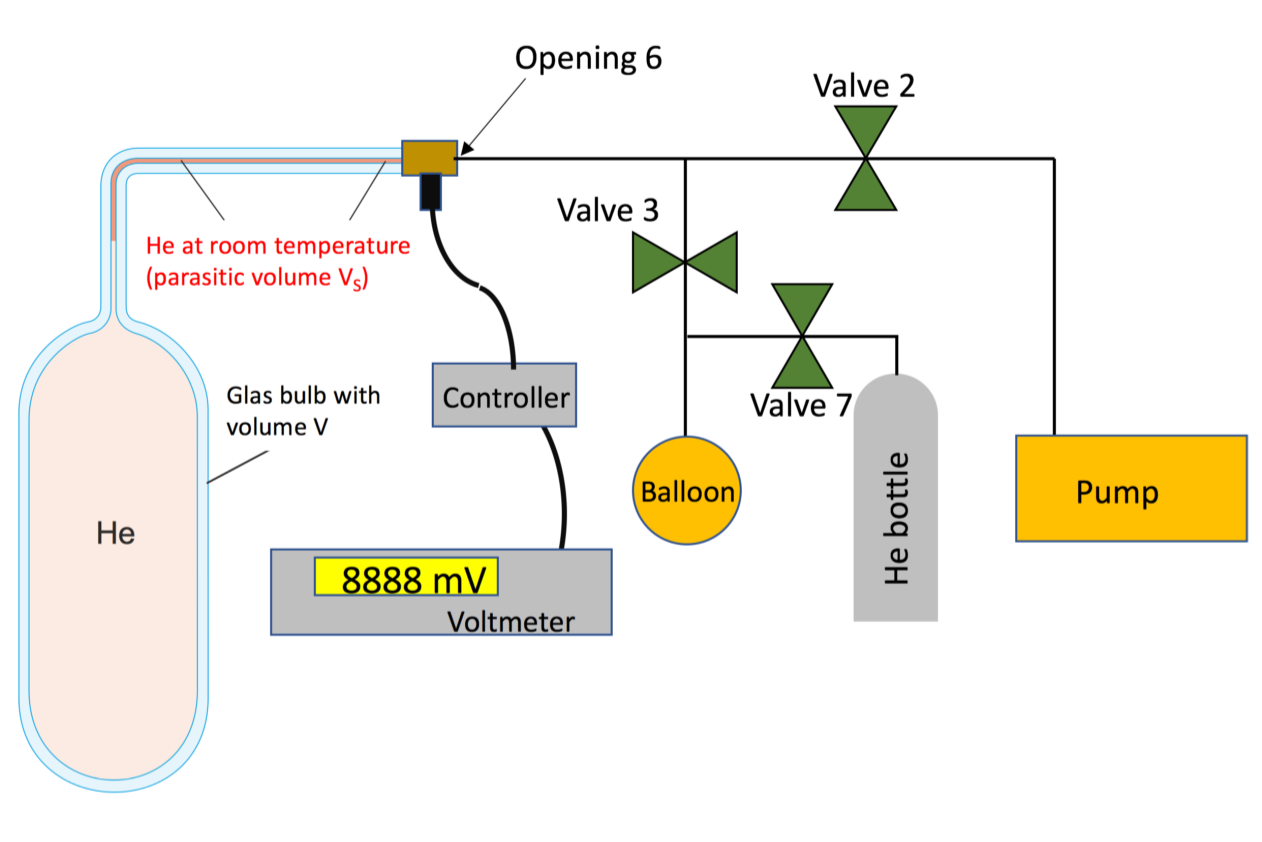
\includegraphics[scale = 0.4]{src/images/experimental_setup.png}
                \caption{\textbf{caption here}}
                \label{fig_setup}
            \end{figure}
        \end{minipage}
        \begin{minipage}{0.5\linewidth}
          \begin{scriptsize}
            \begin{center}
                \begin{figure}[H]
                    \centering
                    \includegraphics[scale = 0.05]{src/images/spectrometer.png}
                    \caption{\textbf{caption here}}
                    \label{fig_spectrometer}
                \end{figure}
            \end{center}
            \end{scriptsize}
        \end{minipage}
      \end{minipage}

    

    \begin{figure}[H]
        \centering
        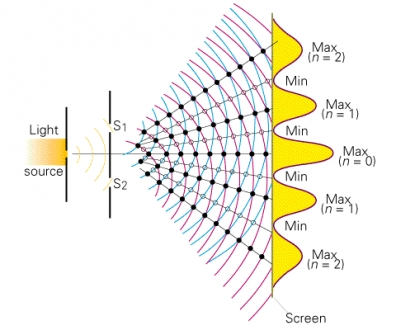
\includegraphics[]{src/images/interference_double_slit.jpg}
        \caption{}
        \label{fig_double_slit}
    \end{figure}

    Light travels in a spherical way behind a slit meaning that each slit acts as a new source of waves
    These waves interfere with each other as they overlap, resulting in an interference pattern of alternating bright and dark regions on the screen or detector.
    This behaviour is due to the fact that two maxima or minima intensify each other while a maximum and a minimum cancel each other out.
    Figure~\ref{fig_double_silt} shows how this effect works.

    \begin{figure}[H]
        \centering
        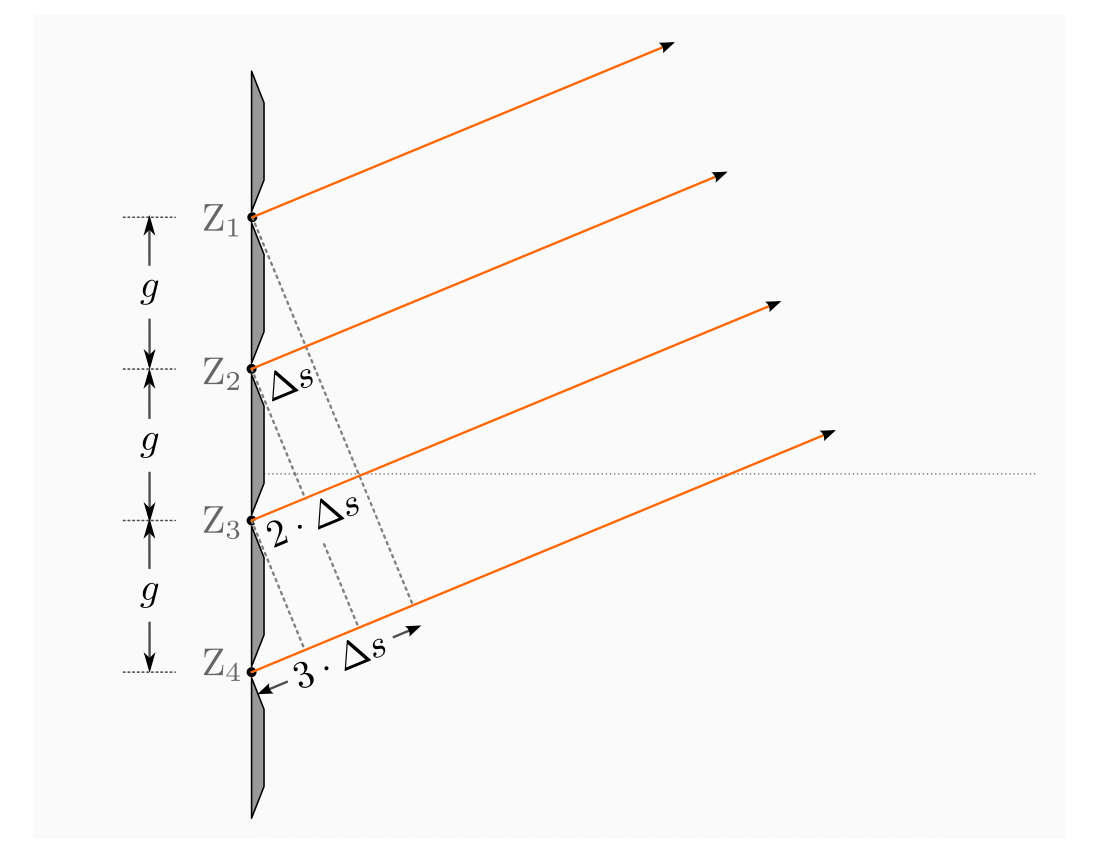
\includegraphics[scale = 0.3]{src/images/interference_grating.png}
        \caption{A grating leads to a similar effect as a double slit.
        $\Delta s$ is equal to the wavelength.
        As seen in the figure, the angle at which brighter spots of light can be seen depends on the wavelength}
        \label{fig_grating}
    \end{figure}
    A grating can be thought of as a lot of slits next to each other and hence it leads to a very similar interference pattern as the double slit.


    % In general this section should tell the reader why he or she should
    % be interested in your paper. Give some background to the
    % experiment, and describe the underlying principles. This is typically where you provide references to previous publications~\cite{Sato2003}.